\chapter{Implementation}
\label{chap:implementation}

\section{Requirements}
    % List and explain the requirements from the specialisation project.
    In the specialisation project leading up to this master's thesis, functional and non-functional requirements were identified. They have been slightly improved in this master's thesis to be clearer and more specific, and one new non-functional requirement (\textbf{nFR6}) have been added explicitly.
    
    \FloatBarrier
    \begin{table}
    \label{tab:fr}
    \caption{Functional Requirements}
    \begin{tabular}{ | c | p{0.9\linewidth} | }
        \hline
        \textbf{ID} & \textbf{Description} \\
        \hline
        FR1 & The Virtual Field Trip (VFT) shall feature a landscape around Vekveselva reconstructed from LiDAR data. \\
        FR2 & The VFT shall use the Virtuix Omni Omnidirectional Treadmill and the HTC Vive Pro Head Mounted Display. \\
        FR3 & The VFT landscape shall have flat areas that the user can walk on.\\
        FR4 & The VFT shall have the ability to transition between a virtual landscape and footage from the real area. \\
        FR5 & The VFT shall project footage either onto spheres or onto the ground, using shaders. \\
        FR6 & The VFT shall contain tasks relevant to the field trip that the player can perform. \\
        FR7 & The VFT shall have a menu where the application can be started, restarted and exited. \\
        \hline
    \end{tabular}
    \end{table}
    \FloatBarrier
    
    \FloatBarrier
    \begin{table}
    \label{tab:nfr}
    \caption{non-Functional Requirements}
    \begin{tabular}{ | c | p{0.9\linewidth} | }
        \hline
        \textbf{ID} & \textbf{Description} \\
        \hline
        nFR1 & The application shall offer at least three of Lazzaro's four fun keys. \\
        nFR2 & The application shall have tasks with intuitive interaction. \\
        nFR3 & The application shall be engaging. \\
        nFR4 & The application shall be fun. \\
        nFR5 & The application shall have good performance, keeping the framerate high enough to not be uncomfortable. \\
        nFR6 & The application shall be based on open source software and tools. \\
        \hline
    \end{tabular}
    \end{table}
    \FloatBarrier

\section{Development Methodology: MVP}
    % A prioritised list of features to be implemented. The first points are regarded as minimum to be completed. Create the list together with domain experts and supervisor.
    The development methodology for creating the \ApplicationName \hspace{0.1cm} is the Minimal Viable Product (MVP) approach. Techopedia\cite{techopedia} defines this at the technique where a product is developed containing the bare minimum functionality. Then, more features are added, typically through feedback produced by the MVP. This technique has two major benefits for this master's thesis. Firstly, it allows users to be included as early as possible in order to better guide the product from an early part of the development when changes are less cumbersome to make. Secondly, it allows for more dynamic planning, as the developer is less experienced in the tools and frameworks necessary to develop the application. This is likely to result in less time used for planning and re-planning due to the uncertainty in time estimates. The plan for the MVP is a prioritised list as can be seen below. The line separates the ''must-have'' features of the MVP from the ''if-time'' features that can be added.
    
    The development also followed a continuous iterative approach. When possible, the application was tested on students to gather feedback. This feedback was used both to improve the features already present, but also to discover new functionality that could be added. The development had no set length for the iterations. This was to, as explained above, focus time on development instead of planning.
    
    \todo{Write more about development methodology}
    
    \setcounter{rownumbers}{0}
    
    \FloatBarrier
    \begin{table}
    \label{tab:mvp}
    \caption{Prioritised List of Features for the Application}
    \begin{tabular}{@{\stepcounter{rownumbers} \therownumbers\hspace*{\tabcolsep}} p{0.9\linewidth}}
        Recreate topology from LiDAR \\
        Re-texture topology \\
        Decorate area with prefabs of trees and grass \\
        Implement image viewer for 360 stereoscopic images \\
        Implement a task for pointing at different parts of the images \\
        \hline
        % Implement a menu for starting and exiting the application \\
        Implement different models for ''Storskredet'' and a way to switch between them \\
        Implement more game mechanics \\
        Improve prefab decorations of the area \\
    \end{tabular}
    \end{table}
    \FloatBarrier

\section{Development Plan}
    % Create a time table with milestones
    To keep tab of the progress, the following development plan with milestones was used:
    
    \FloatBarrier
    \begin{table}
    \label{tab:plan}
    \caption{Plan with Milestones for the Project}
    \begin{tabular}{| p{0.2\linewidth} | p{0.725\linewidth} |}
        \hline
        \textbf{Time} & \textbf{Milestone} \\
        \hline
        End of January & Finalise the shape of the terrain and finish the MVP feature list \\
        End of February & Finish decorating the area with prefabs, incorporate image viewing and decide on game mechanics to be used in cooperation with domain experts \\
        End of March & Implement game mechanics \\
        14th of April & Finish prototype development and freeze code. Finish questionnaires for testing and tasks for the Penn State application. \\
        End of April & Finish user testing with students and finish interview questions for domain experts \\
        15th of Mai & Finish user testing, interviewing domain experts and finish comparison of applications \\
        10 of June & Finish structuring and analyse collected data, finalise the project and the report, export any assets that can be reused by IMTEL \\
        \hline
    \end{tabular}
    \end{table}
    \FloatBarrier

\section{Creating the Ground Model}
    \label{sec:recreating_ground}
    % Kartverket    - acquire point cloud
    % LasTools      - merge files
    % LasTools      - filter vegetation
    % LasTools      - convert to .txt
    % Meshlab       - import .txt
    % Meshlab       - recreate normals  (normal recreation)
    % Meshlab       - recreate topology (screened poisson surface)
    % Meshlab       - simplify          (MC edge collapse)
    % Meshlab       - cleaning          (remove duplicate vertices and faces)
    % Meshlab       - set origin        (transform, set origin)
    % Meshlab       - export .ply
    % Blender       - import .ply       (viewport must be adjusted)
    % Blender       - cut model         (Blender nearly crashes at this point, loads unresponsive for 20+ seconds, not done in Meshlab because want other than square regions)
    % Blender       - export .ply
    % Meshlab       - import .ply
    % Meshlab       - simplify          (quadratic edge collapse decimation 0.01 on area and 0.001 on surroundings)
    % Meshlab       - export .ply
    % Blender       - import .ply
    % Blender       - rework walkway    (curve, box, edit box, array box, curve box, shrinkwrap)
    % Blender       - texture models    (materials, image brush)
    % Blender       - export .fbx and texture image
    % Unity         - import .fbx and texture image
    As explained more in detail in the Specialisation Project\cite{specialisation}, the topology was recreated from LiDAR scans of the area, publicly available at Kartverket\cite{hoydedata}. The complete pipeline for creating a usable model for the ground, without sacrificing too much performance, has many steps. In order to get an overview of the process, as well as details and reasoning, the pipeline is presented as a numbered list in \cref{tab:pipeline}, followed by sections detailing the steps. The numbered list also contains a column showing which software or service is used in each step.
    
   The reconstruction pipeline is based on the Specialisation Project which is again based on the master's thesis by Staurset\cite{ski_jump}. The pipeline has been expanded and more thoroughly detailed to provide a better overview of the process.
    
    \setcounter{rownumbers}{0}
    
    \FloatBarrier
    \begin{table}[htbp]
        \centering
        \caption{Reconstruction Pipeline Steps}
        \label{tab:pipeline}
        \begin{tabular}{| c | c | p{0.575\linewidth} |}
            \hline
            \textbf{Number} & \textbf{Software / Service} & \textbf{Description} \\
            \hline
            \rownumber & Kartverket\footnote{The Norwegian Mapping Authority} & Acquire point cloud in \texttt{.laz} files \\
            \rownumber & LasTools & Merge the \texttt{.laz} files into one \\
            \rownumber & LasTools & Filter out the vegetation from the \texttt{.laz} files \\
            \rownumber & LasTools & Convert \texttt{.laz} file to \texttt{.txt} file \\
            \rownumber & Meshlab & Recreate normals for points \\
            \rownumber & Meshlab & Recreate surface \\
            \rownumber & Meshlab & Simplify (decimation) and cleaning \\
            % \rownumber & Meshlab & Set origin \\
            \rownumber & Meshlab & Export model as \texttt{.ply} file \\
            \rownumber & Blender & Cut model into smaller parts\\
            %\rownumber & Blender & Export models as \texttt{.ply} files \\
            %\rownumber & Meshlab & Simplify (decimation) and cleaning \\
            %\rownumber & Meshlab & Export models as \texttt{.ply} files \\
            %\rownumber & Blender & Rework walkway model \\
            \rownumber & Blender & Texture models \\
            \rownumber & Blender & Set origin \\
            \rownumber & Blender & Export models as \texttt{.fbx} files \\
            \hline
        \end{tabular}
    \end{table}
    \FloatBarrier
    
    \subsection{Acquire Point Cloud from Kartverket}
        The first step of creating the ground model is to acquire the LiDAR scans of the area. The scans are openly available at the Norwegian Mapping Authority - Kartverket. On their web pages, the area in question can be marked and the data files will be made available at a custom link address. Depending on the size of the area, the data will typically be divided into several \texttt{.laz} files.
        
        It could also be possible to get terrain models directly from Kartverket. One would then have to find software to open the model files (\texttt{geoTiff}) and find another way to filter out the vegetation.
    
    \subsection{Filter with LasTools}
        LasTools\cite{lastools} is a semi-open source software developed by rapidlasso. It has several functions to work on point cloud data, where some are completely open source, and others are free to use for non-commercial projects.
        
        With the \texttt{.laz} files available, the most practical thing is to merge the files into one. Afterwards, the terrain can be filtered from the vegetation using one of the only-for-non-commercial functions: \texttt{lasground\_new.exe}. Finally, the point cloud can be exported as a \texttt{.txt} file that Meshlab can read.
    
    \subsection{Simplify and Reconstruct Surface with Meshlab}
        The software used for the surface recreation is Meshlab\cite{LocalChapterEvents:ItalChap:ItalianChapConf2008:129-136}. The software is open source and made for working with large point clouds and models, as well as supporting mesh reconstruction. %Although it could be a good idea to reduce the size of the point cloud, the model contains a walkway in the valley that is important to keep as precise as possible.
        In order to reduce the complexity of the ground model, the point cloud was sub-sampled outside of the important area, the river and the walkway. It was sub-sampled to be about 1 point per 1 model unit in Meshlab.
        
        \FloatBarrier
        \begin{figure}[htbp]
            \centering
            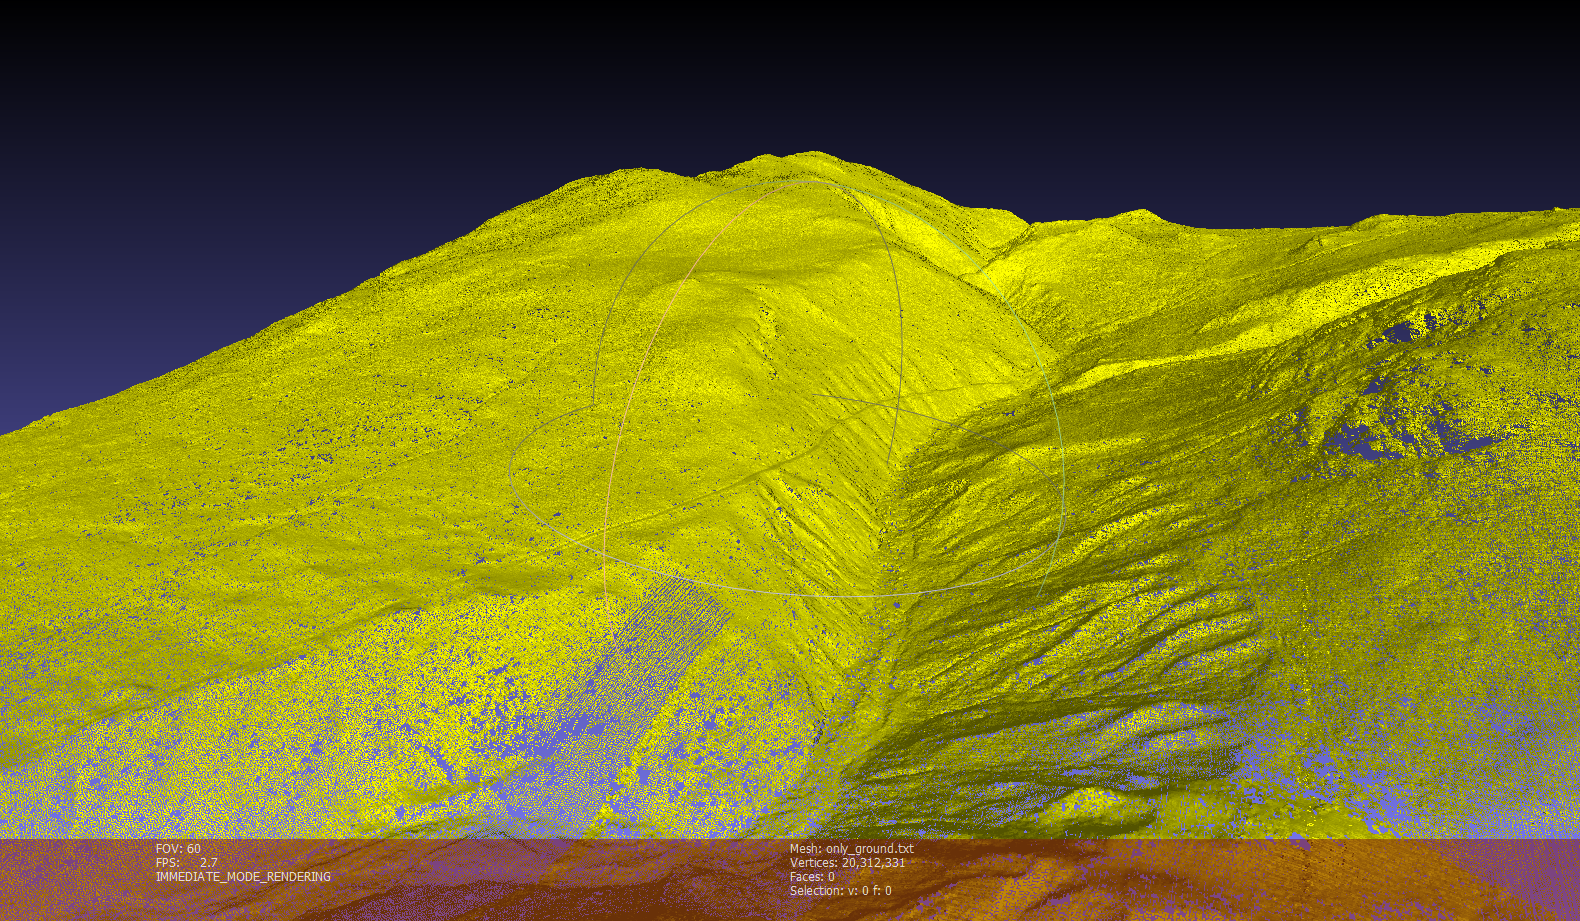
\includegraphics[width=\ImageWidth]{figures/point_cloud.PNG}
            \caption{Filtered Point Cloud for the Ground in the Vekveselva River Area}
            \label{fig:point_cloud}
        \end{figure}
        \FloatBarrier
        
        Screened Poisson Surface Reconstruction\cite{kazhdan2013screened} was used to recreate the ground model from the point cloud. It relies on the points having normals, so these normals had to be calculated first. The reconstructing algorithm was tested with different reconstructing depths where the choice landed on 12. This resulted in longer computing time but a good reconstruction quality. The model was also cleaned for duplicate edges and vertices without normals. Afterwards it was exported as \texttt{.ply} file.
        
        %Because the ground model is constructed from points, and the points have gps coordinates, the resulting model has a very large offset from its local origin. Although a better practise would be to keep these coordinates, as they could be useful information later, they made it hard to locate the model in programs like Blender. Therefore the origin of the model was reset to approximately the centre of the geometry. The model was exported as a \texttt{.ply} file as it can be read by both Blender and Meshlab and has good compression.
        
    %\subsection{Simplify Model in Meshlab}
        %With the model divided into different parts, they can be simplified tailored to their importance. The Quadratic Edge Collapse Decimation algorithm was used to achieve this. This simplification allows to preserve the general topology, as well as the edges of the final model. This is important as the different parts of the model need to fit together at the end. The simplification was controlled by stating the percentage of vertices that should survive. Different percentages was tested for the ground models, to trade off quality against file size. As the models had a very high vertex count, the walkway was scaled to 15 \% of original vertex count, the main area was set to 2 \% and the rest were set to 0.1 \%. In \cref{fig:post_simplification} this simplification is most visible in the outer area.
        
    
    \subsection{Cut the Model in Blender}
        Blender\cite{blender} is a versatile, open source software with many different features. It was used to further rework and texture the model where Meshlab proved less appropriate. It was first used to partition the model into three areas to be used for different purposes. This partitioning can be seen in \cref{fig:model_original}.
        %The reasoning behind the partition is to cut the model into the part that the player will move on, the are they will look at most, and the part they are only supposed to view at a distance or not at all. This will also allow parts of the model to be worked on in isolation from the rest.
        This partitioning allows for reworking the area the player will walk on and also to switch out the model for the Storskredet landslide. It also allows to define a game area for teleporting, and have a water tight mesh collider for areas where other models will be swapped in.
        
        \FloatBarrier
        \begin{figure}[htbp]
            \centering
            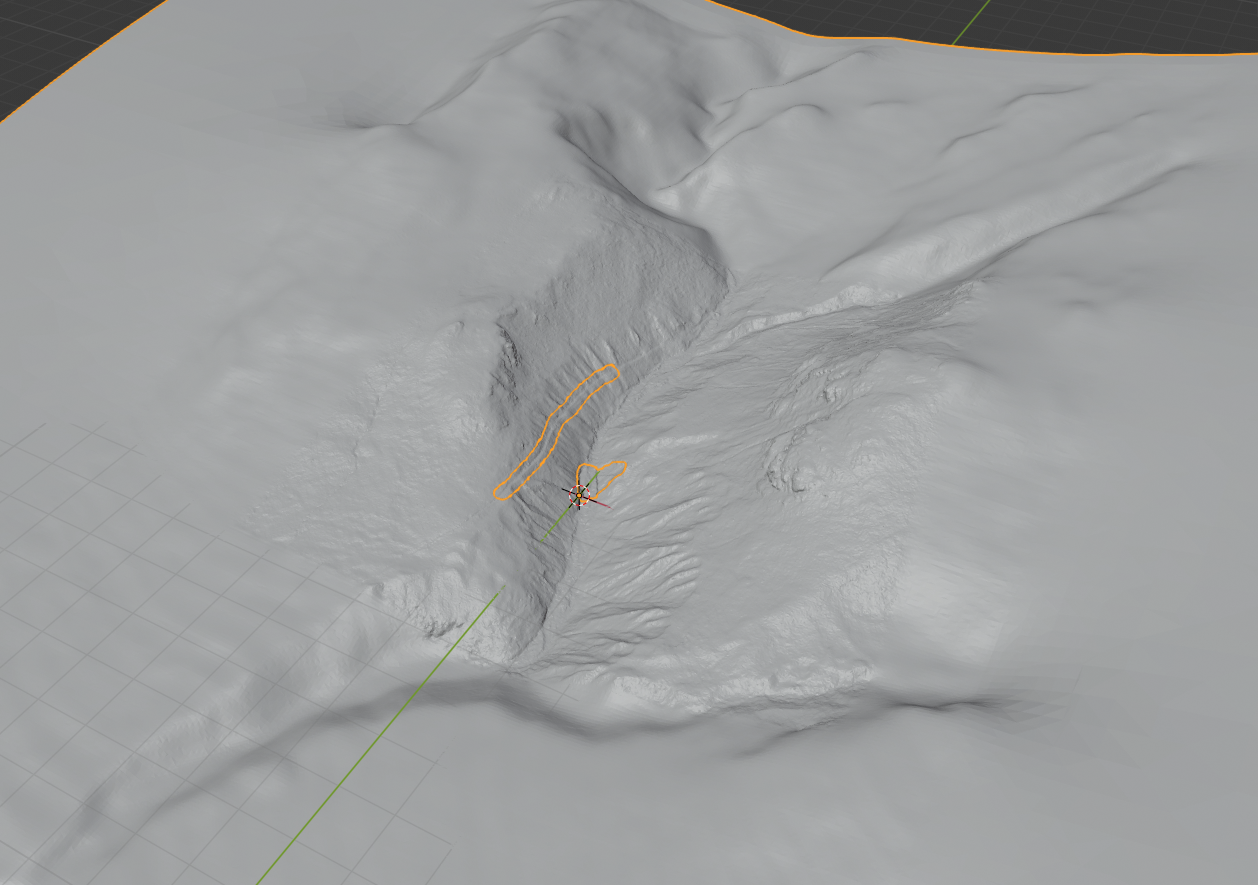
\includegraphics[width=\ImageWidth]{figures/ground_simplified_cut.PNG}
            \caption{Partitioning of the Ground Model After Simplification}
            \label{fig:model_original}
        \end{figure}
        \FloatBarrier
    
    \subsection{Texture Model and Set Origin in Blender}
        %Although the recreation of the walkway was successful, the omnidirectional treadmill needs more space than a person would normally need. This is because it is less precise than actual walking, as well as a little harder to control. To accommodate this the walkway was reworked in Blender to provide a flatter surface for the players.
        The ground model was textured using a satellite image from Google Maps. The texture ground can be seen in \cref{fig:ground_textured} below. Afterwards the origin of the model was moved. This needed to be done because the vertex coordinates from the LiDAR point cloud was still preserved in the model, placing the actual topography some 7000 kilometres from the model's origin. The models were offset $[x, y, z] = [-530447, -6945400, -854]$. This offset was applied to all models so they could still be automatically placed relative to one another. The coordinates of the point cloud were in \textbf{UTM 32N} with \textbf{EPSG 25832}. Finally the ground models were exported as \texttt{.fbx} files, as Unity does not support the \texttt{.ply} format.
        
        \FloatBarrier
        \begin{figure}
            \centering
            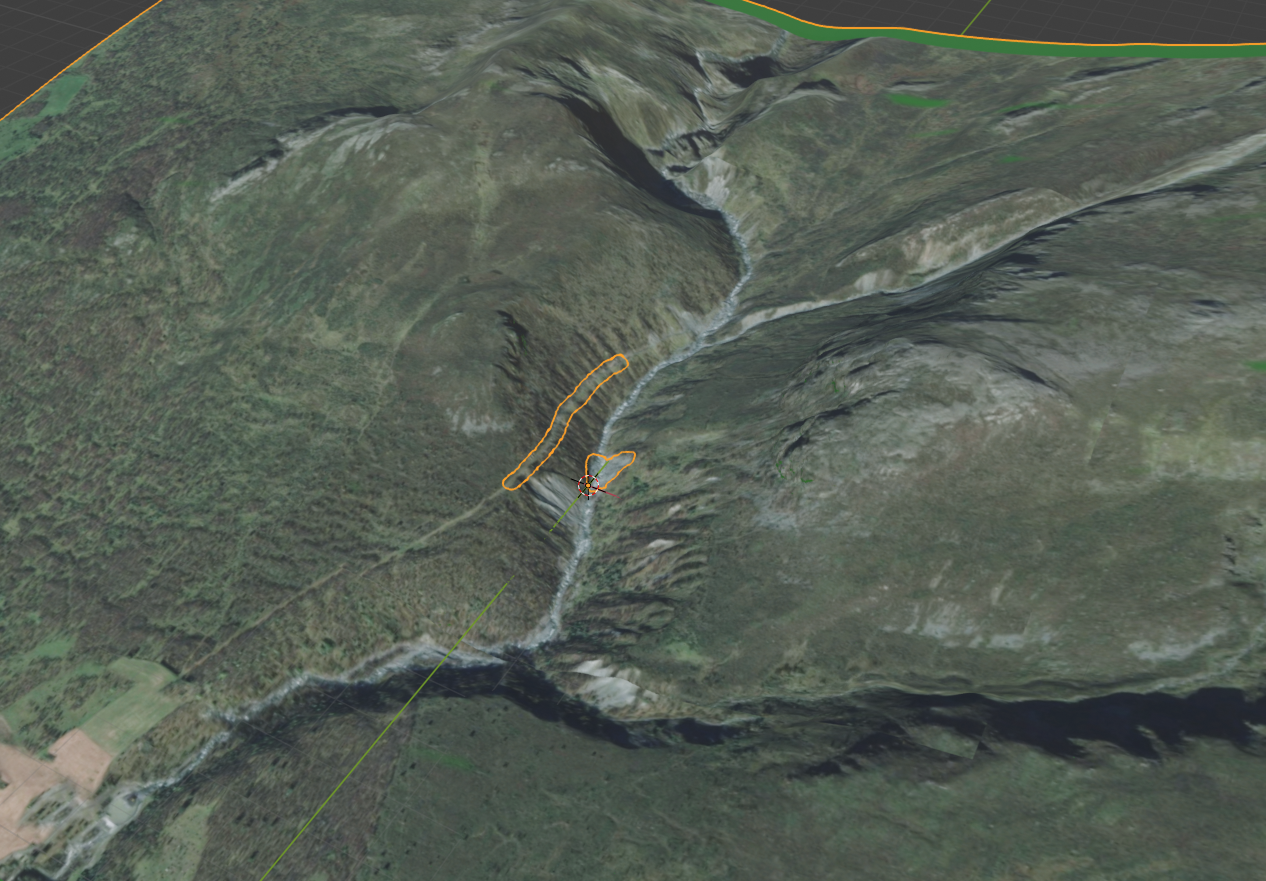
\includegraphics[width=\ImageWidth]{figures/ground_textured.PNG}
            \caption{Ground Textured with Satellite Imagery}
            \label{fig:ground_textured}
        \end{figure}
        \FloatBarrier
        
        
        \begin{comment}
        
        \FloatBarrier
        \begin{figure}[htbp]
            \centering
            \begin{minipage}[b]{0.4195\textwidth}
                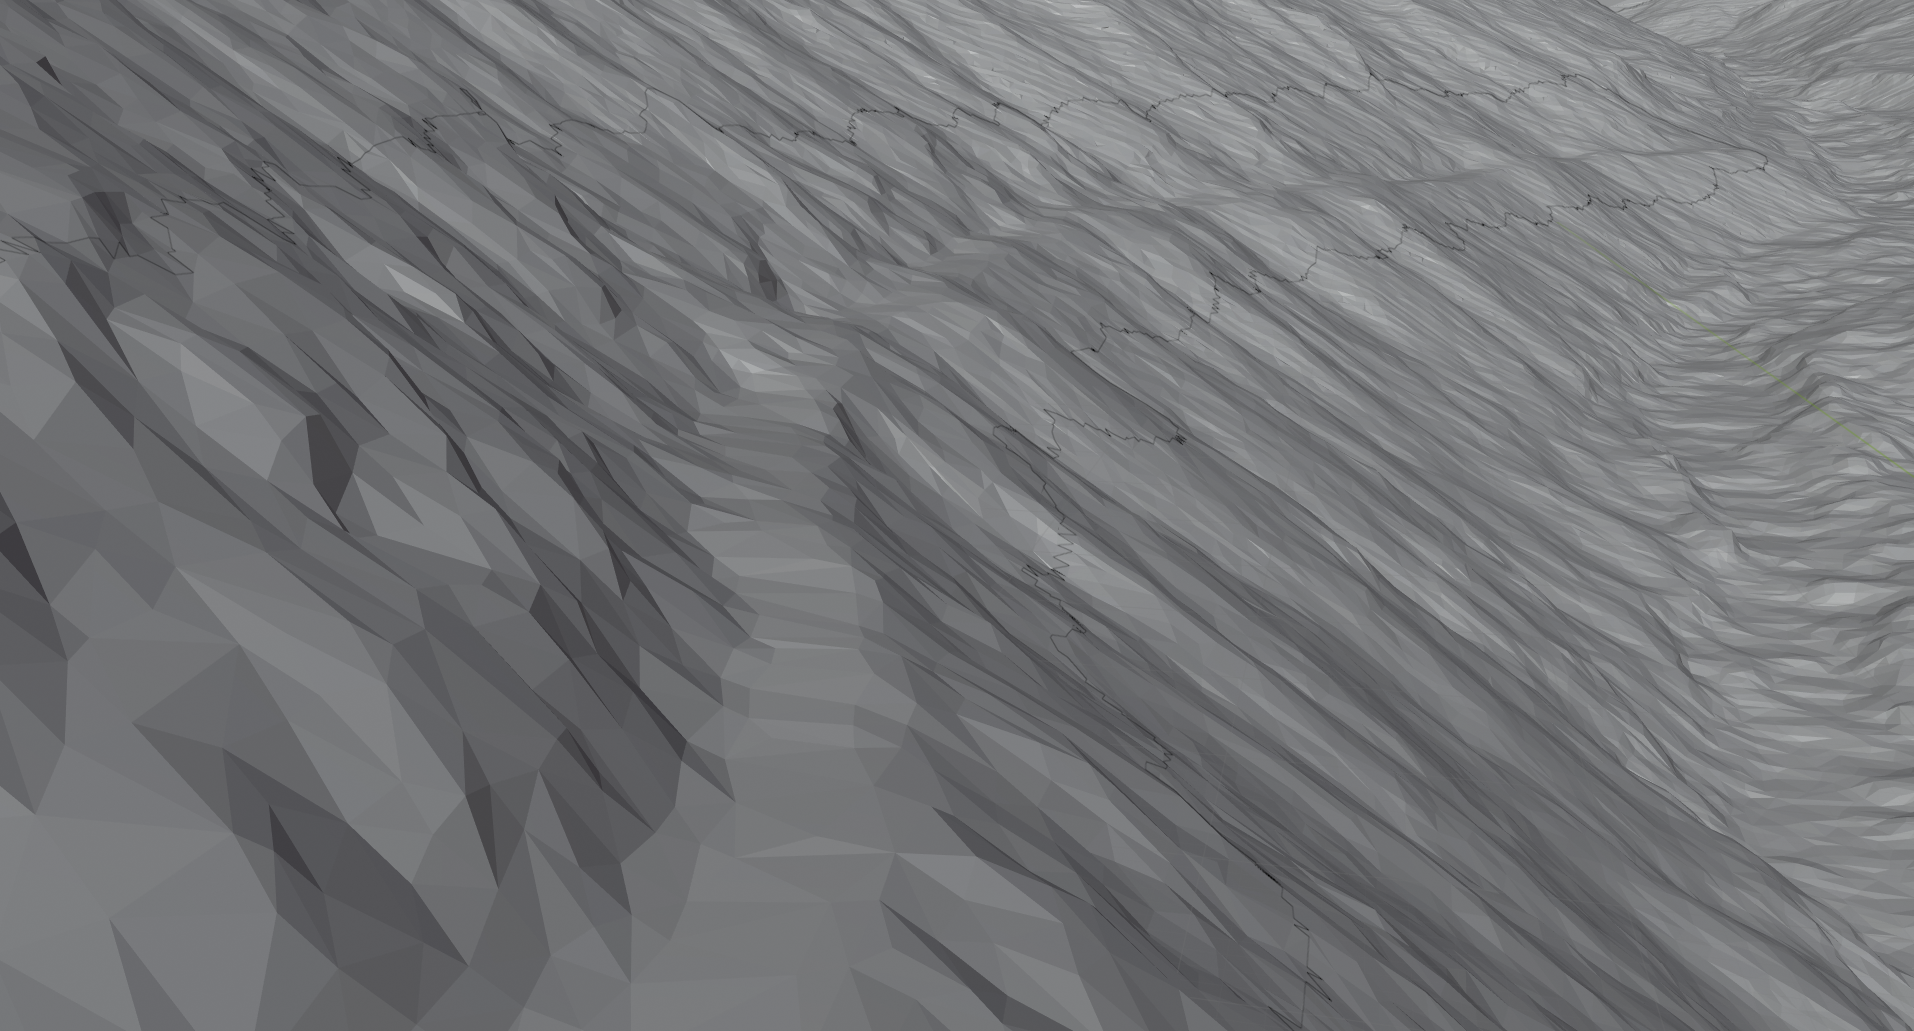
\includegraphics[width=\textwidth]{figures/walkway_before_rework.PNG}
                \caption{Walkway Before Rework}
            \end{minipage}
            \begin{minipage}[b]{0.4\textwidth}
                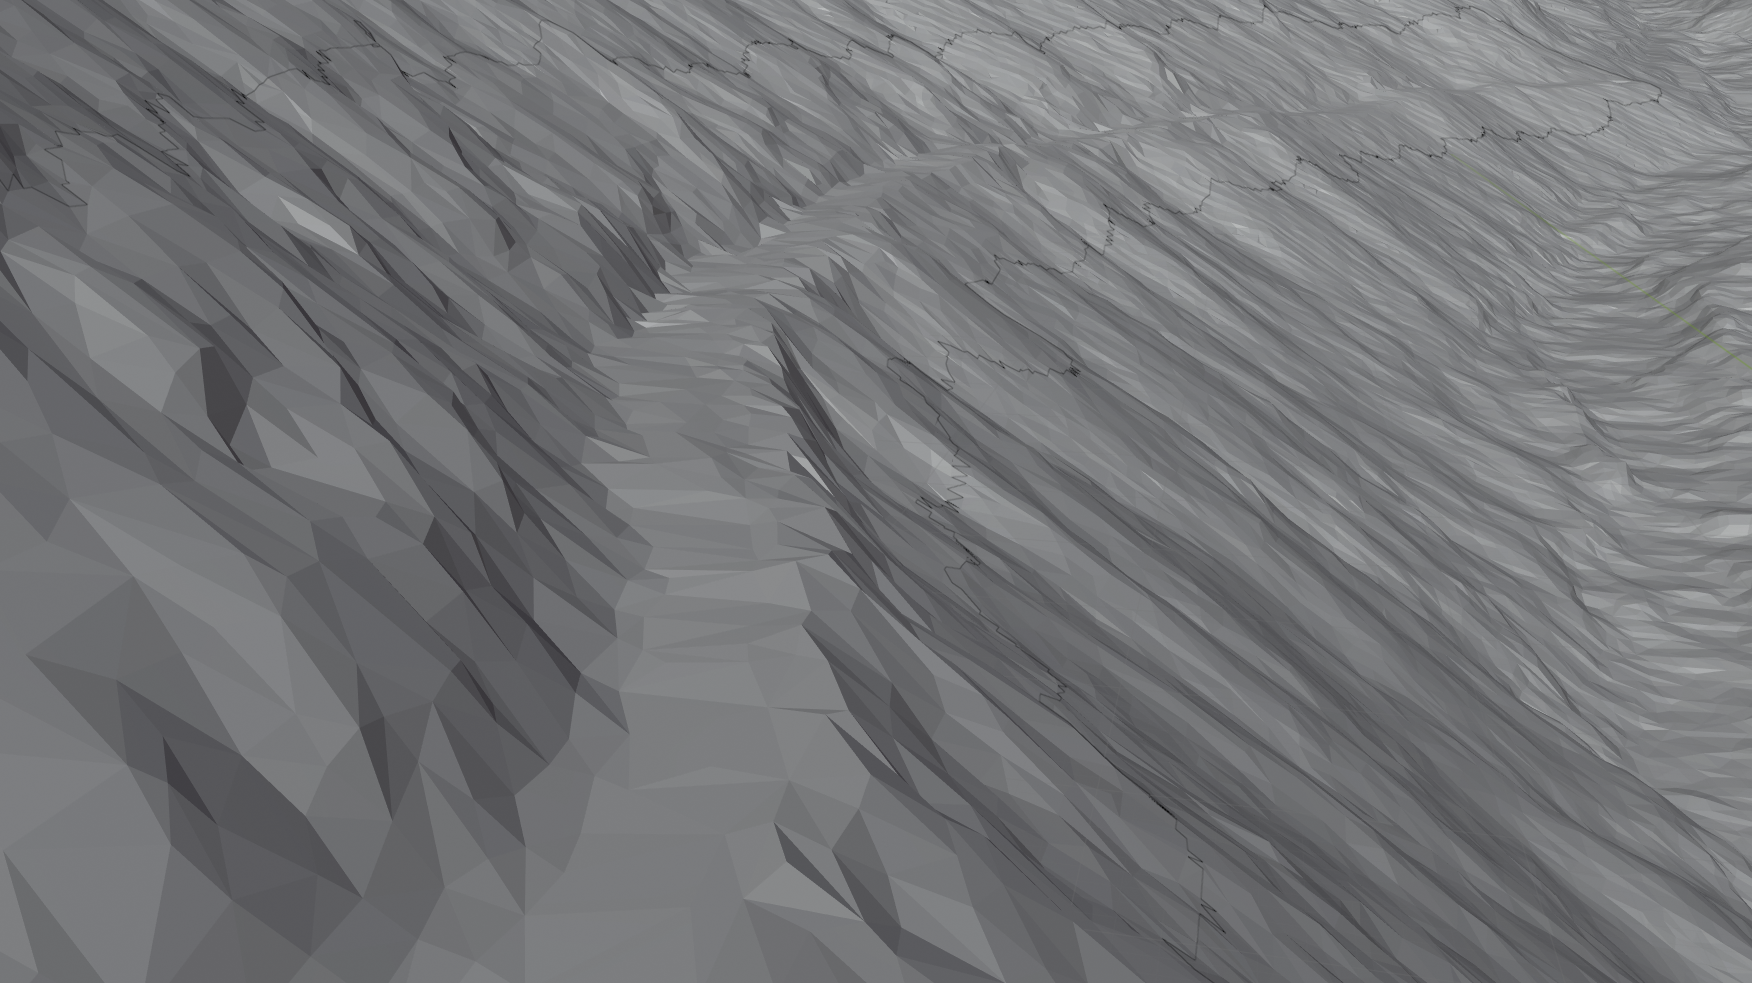
\includegraphics[width=\textwidth]{figures/walkway_after_rework.PNG}
                \caption{Walkway After Rework}
            \end{minipage}
        \end{figure}
        \FloatBarrier
        
        \end{comment}

\section{Implementation in Unity}
    % How stuff was made in Unity, potentially code snippets.
    \subsection{Overall Architecture}
        % Class diagram
        % Component interaction
        % Preload scene, dontdestroyonload
        % Extending/inheriting existing scripts
        The main building blocks of Unity are \textit{scenes}. These are individual hierarchies of \textit{transforms}, where the transforms in turn have different \textit{components} attached to them. All the objects in a scene are therefore transforms with components, structured in the scene graph hierarchy. The scene graph and components, like Image Viewer and Object Spawner, attached to the ''Walkway11'' transform can be seen in \cref{fig:unity} below.
        
        \FloatBarrier
        \begin{figure}
            \centering
            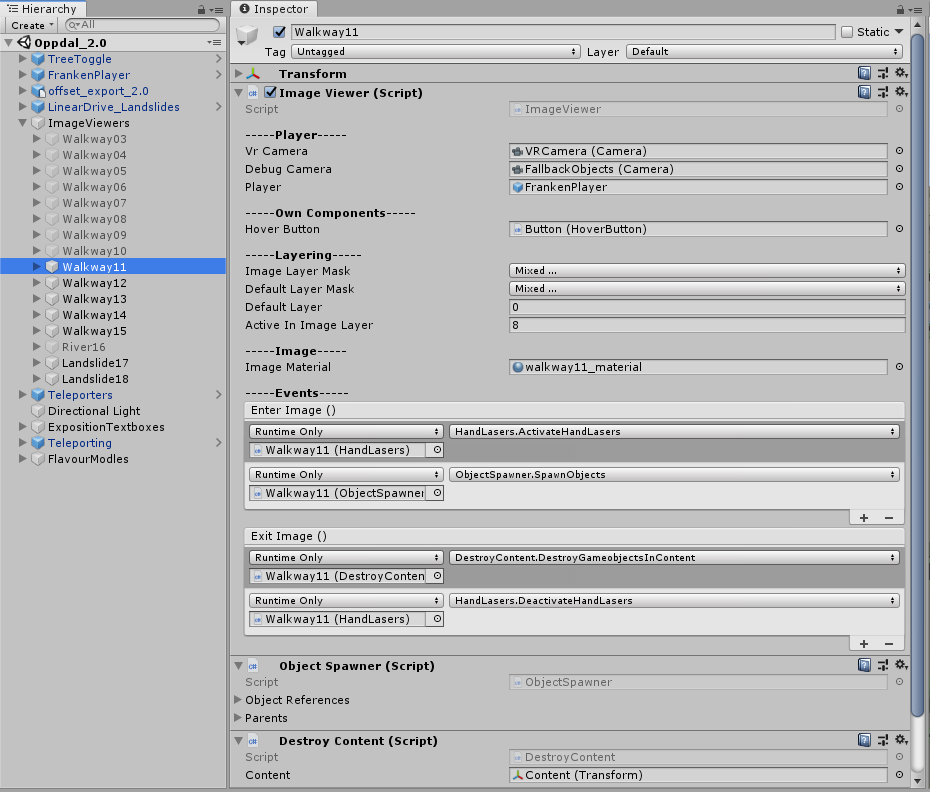
\includegraphics[width=\ImageWidth]{figures/unity.PNG}
            \caption{Left: Hierarchical Scene Graph, Right: Components Attached to the Selected Transform}
            \label{fig:unity}
        \end{figure}
        \FloatBarrier
        
        Because of the way Unity is structured, it is highly recommended to use \textbf{component oriented} code. This means that code features are loosely coupled and therefore easier to change and reuse. This can be seen in the image above where the components are stand-alone features that are attached to the transform, instead of being hard-coded. Unity has three main ways of supporting the component oriented approach:
        
        \begin{itemize}
            \item \textbf{Components} \\
            As described, components are added to transforms to make up the different objects in the scene graph.
            
            \item \textbf{Linking} \\
            Transforms, and their components, can be linked to components. This can be seen in the Image Viewer component in \cref{fig:unity} were transforms like VR Camera have been linked. The transforms can also be searched by name or type in scripts.
            
            \item \textbf{Events} \\
            Functions without input parameters or return values can be linked and triggered by events, as seen in \cref{fig:unity} in the Image Viewer component. This allows for components to be loosely coupled to each other without the need for hard-coding their interactions.
        \end{itemize}
        
        The main connections between the different components can be seen below in \cref{fig:component_interaction_diagram}. These connections form the main gameplay mechanics of the application.
        
        \FloatBarrier
        \begin{figure}
            \centering
            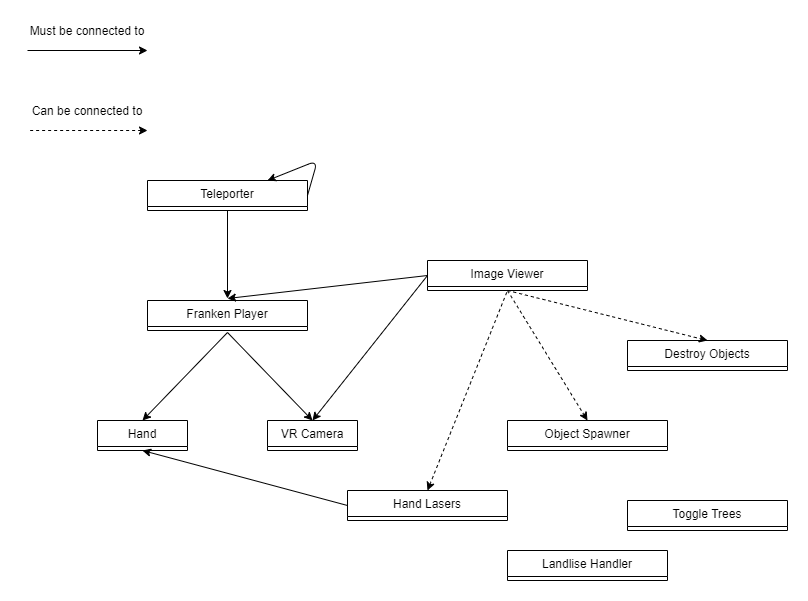
\includegraphics[width=\ImageWidth]{figures/component_interaction_diagram.png}
            \caption{Component Interaction Diagram}
            \label{fig:component_interaction_diagram}
        \end{figure}
        \FloatBarrier
        
        The interaction can be divided into five main areas:
        
        \begin{itemize}
            \item \textbf{The Player} \\
            This is the object necessary for movement, looking around with the VR camera and viewing and using the hands. This is the largest and most complicated object, but has been simplified as it has many internal workings.
            
            \item \textbf{The teleport} \\
            The teleporter is very simple object in the application, but requires linking to the player to be able t move it.
            
            \item \textbf{The Hand Lasers} \\
            This component needs to be linked to the hands of the player in order to activate and deactivate the laser pointer objects native to the hands. It also activates and deactivates logic that allows the pointers to activate other objects.
            
            \item \textbf{The Image Viewer} \\
            These are the main gameplay mechanics and have to be linked to the player and camera in order to set the culling mask and change the view for the player. It also sets of events when entering and exiting image mode, allowing game world modifiers to be attached if wanted.
            
            \item \textbf{Game World Modifiers} \\
            These are simple objects that manipulate the game world itself without the need for integration with the other main objects. They create, destroy, activate and deactivate parts of the game world.
        \end{itemize}
    
    \subsection{The Player}
        % Add treadmill to SteamVR player
        % Add teleport functionality for use without treadmill
        The player object was created by combining two existing player prefabs from Steam VR and the Omni SDK. The player from Omni SDK is focused on using the Virtuix Omni omnidirectional treadmill as movement input, whereas the Steam VR player has a lot of built-in support for the hand controllers, but is meant to be standing still. The new player was created by adding the Steam VR player as a child in the Omni player and deleting the original VR camera in the Omni player, as there is already one present in the Steam VR player. It can be compared to simply placing the Steam VR player ''on wheels''. This resulted in a player controlled by the Virtuix Omni, but with all the support and integration of the Steam VR player, like adding teleportation as an alternative mode of transportation if a treadmill is unavailable.
        
        \todo{Include image of hierarchy combination?}
    
    \subsection{Viewing Stereoscopic 360 Images}
        In order to view the stereoscopic 360 images, the tutorial of Heavers\cite{skybox_images} was followed. This solution uses a custom shader to project the images to the skybox of the game world. This method can be used by loading a new empty scene with the custom skybox or change the skybox of the main world. The latter way was chosen in an effort to reduce load time when activating the image mode. When activating the image mode, the rest of the game world is hidden from the player, and the skybox material is changed to the appropriate image.
        
        To control what was to be masked and what was to be shown in the image mode, layers and culling masks were used. The culling mask is a feature in Unity cameras that determines which layers are visible and not. The objects that should be visible were assigned the ''ActiveInImage'' layer. This meant that some objects, like the buttons for toggling image mode, had to be assigned layers at runtime. This also required some changes in Steam VR resources as it had not implemented layers as a part of e.g. spawning hand models or using laser pointers. The activation button can be seen under in \cref{fig:image_viewer}.
        
        \FloatBarrier
        \begin{figure}
            \centering
            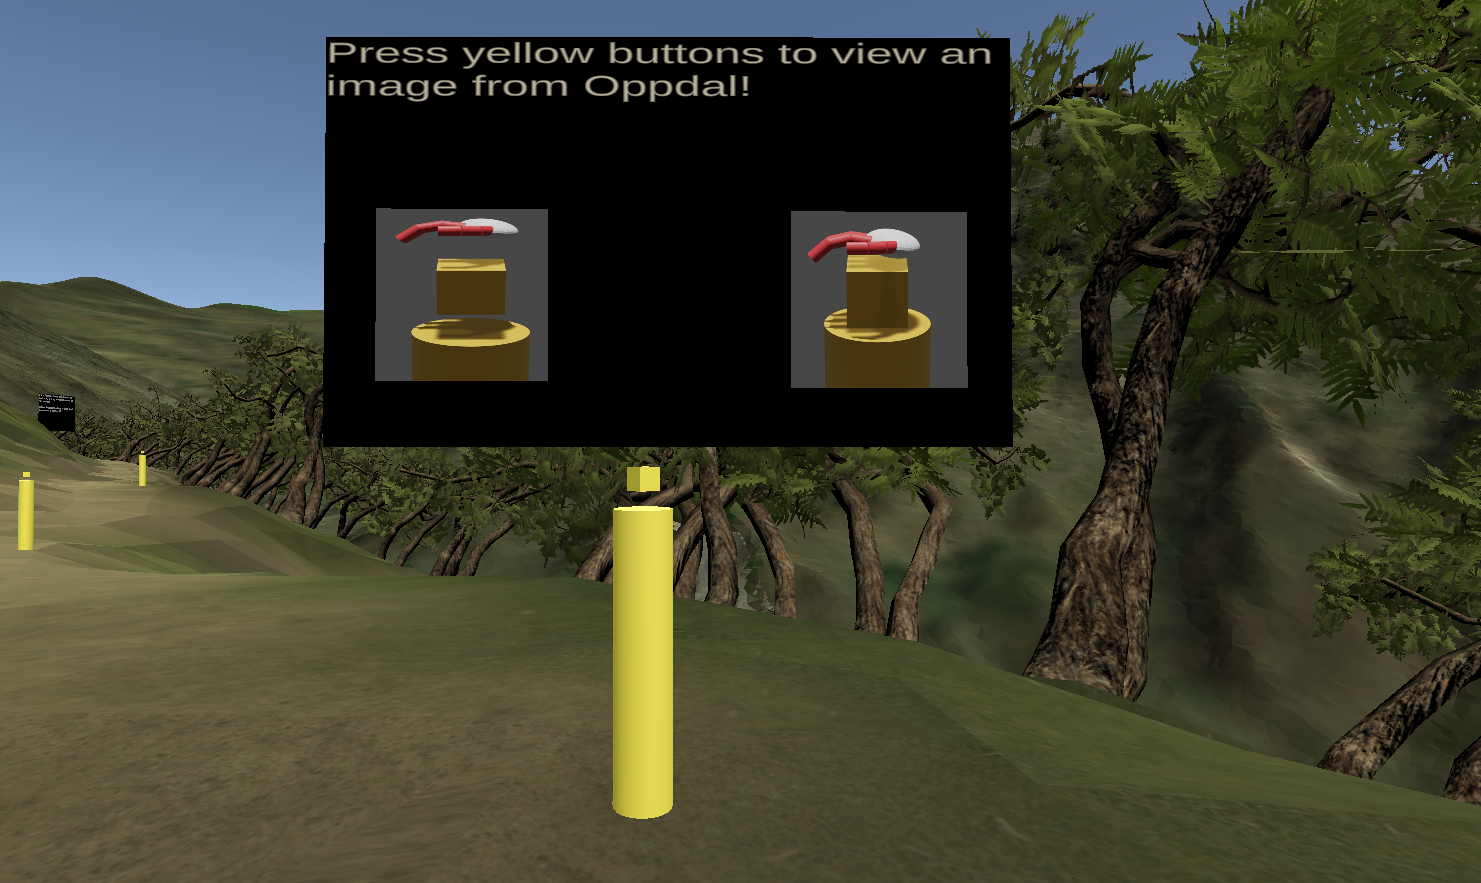
\includegraphics[width=\ImageWidth]{figures/image_viewer_3.PNG}
            \caption{Button for Toggling Image Mode}
            \label{fig:image_viewer}
        \end{figure}
        \FloatBarrier
        
        \todo{Screenshot video without scene view}
        
    \subsection{Point-and-Click Tasks}
        In order to engage the players, point-and-click tasks were created. These tasks were activated while in ''image mode''. As the tasks are component based, they could also be used outside of the image mode, but that could be problematic when the player can move around. The task were made textboxes, Steam VR laserpointers and simple plane objects. The textboxes instructed the player on what to point at. The Laserpointers visualized the pointing and activated components on the planes. The planes were placed to cover the area of the image that should be pointed at and was then turned invisible. The planes were shown with a highlighter around its edge after it was activated by the user. The Steam VR laserpointers required some reworking to be able to see through certain objects.
        
        \FloatBarrier
        \begin{figure}[htbp]
            \centering
            \begin{minipage}[b]{0.45\textwidth}
                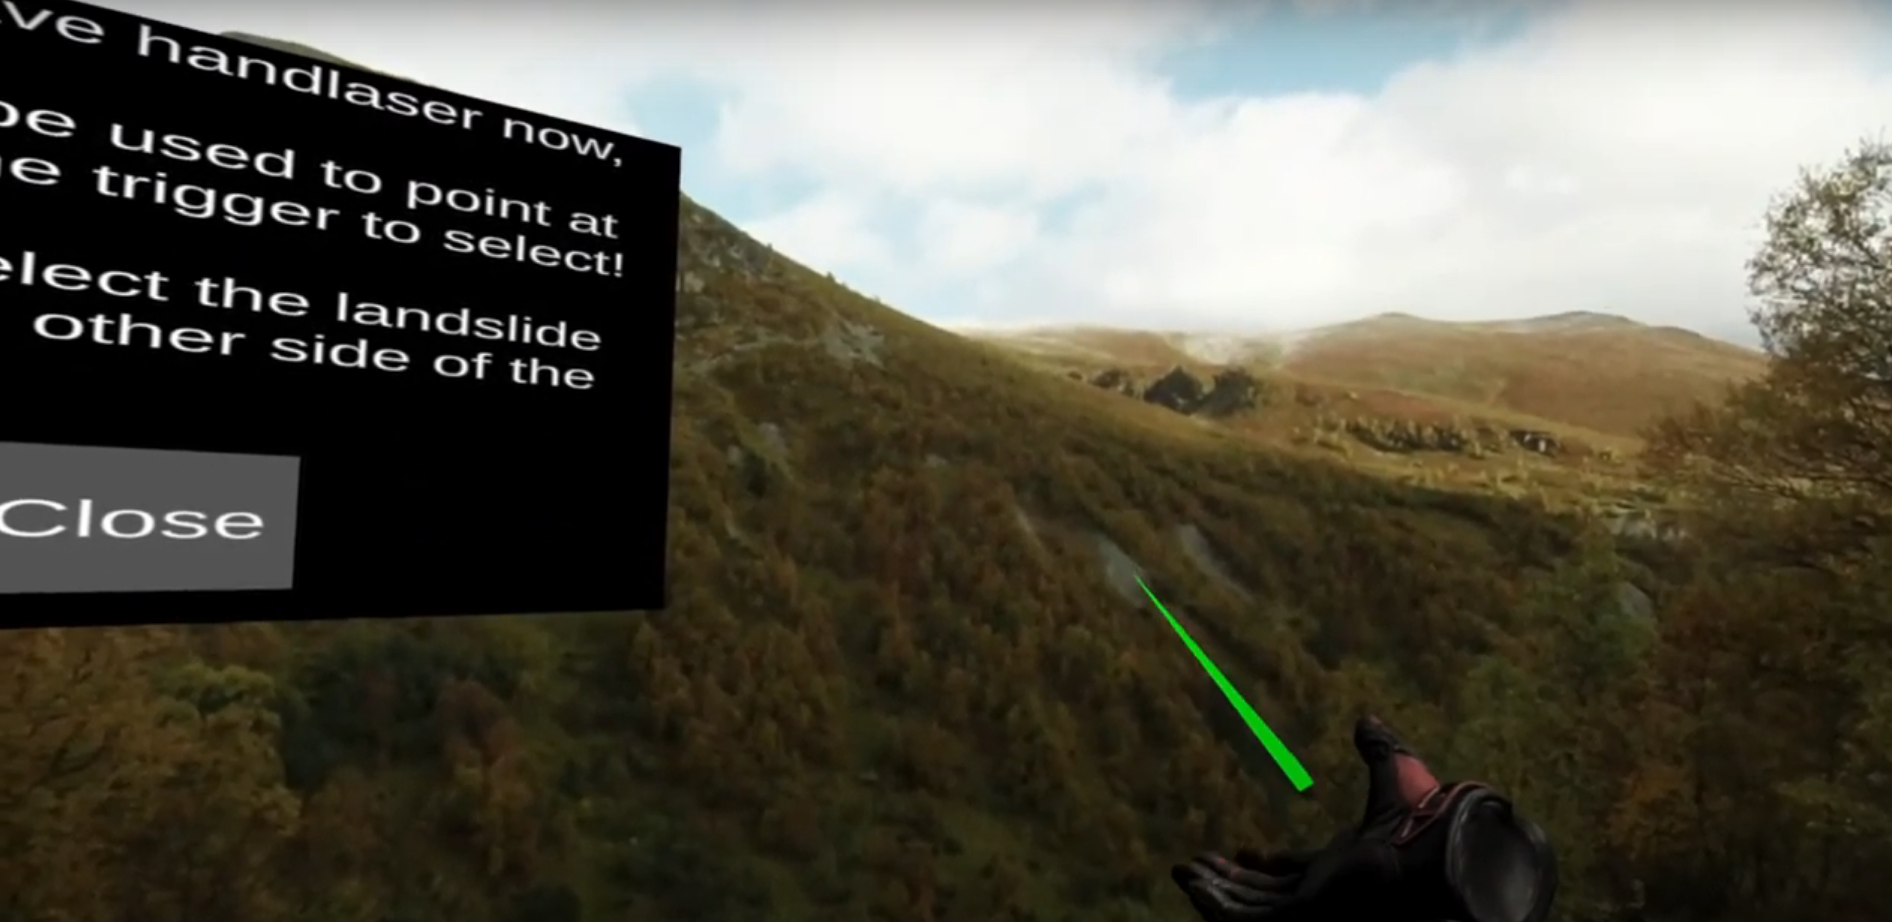
\includegraphics[width=\textwidth]{figures/point_and_click.PNG}
                \caption{Player Pointing}
            \end{minipage}
            \begin{minipage}[b]{0.45\textwidth}
                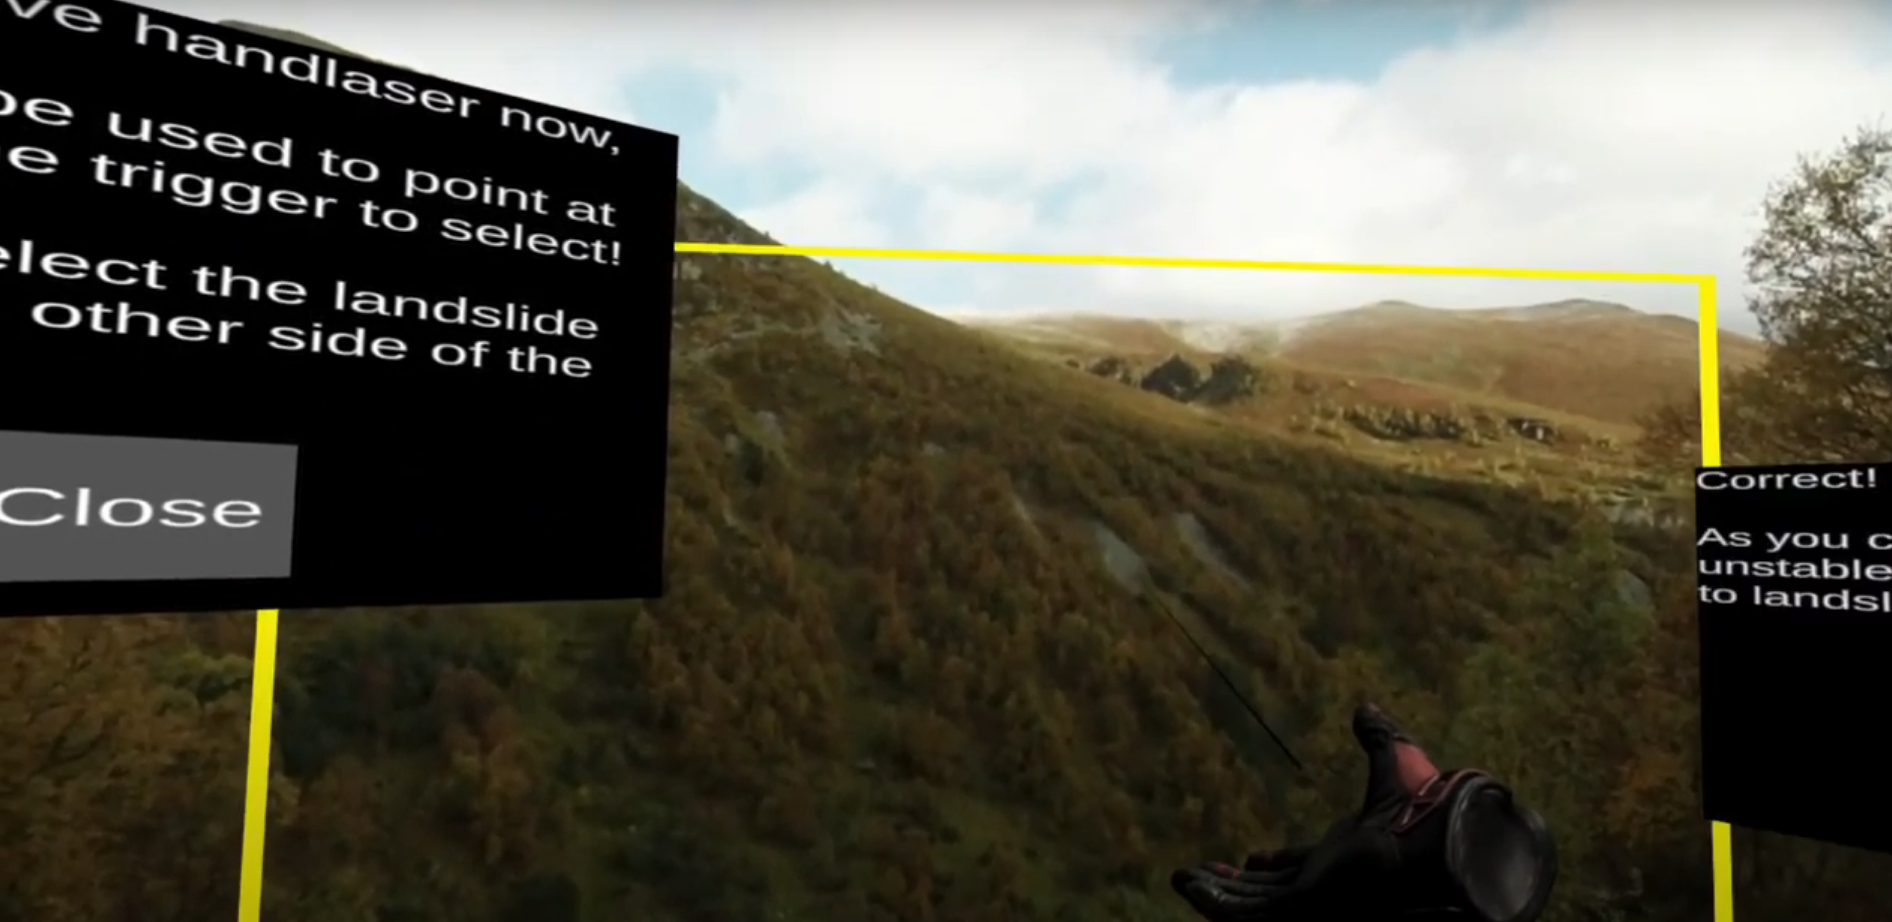
\includegraphics[width=\textwidth]{figures/point_and_click_clicked.PNG}
                \caption{Player Clicked}
            \end{minipage}
        \end{figure}
        \FloatBarrier
    
    \subsection{Different Landslide Models}
        A tradition of the actual field course it to scan one of the landslides in the area with LiDAR. These scans have been used in software to analyse the development of the landslide. Because of this there were several point clouds of the landslide available to be reconstructed and included in the application. They were reconstructed in the same way as the ground model in \cref{sec:recreating_ground}, having the same offset to be placed automatically. The landslides could then be toggled by setting their active status to true or false.
        
        The interface for selecting the landslide models was a linear drive with a shaft and table from Steam VR. The input of the linear drive was then used to activate the landslides, depending on it's position. The interface can be seen below in \cref{fig:landslide_handler}:
        
        \FloatBarrier
        \begin{figure}
            \centering
            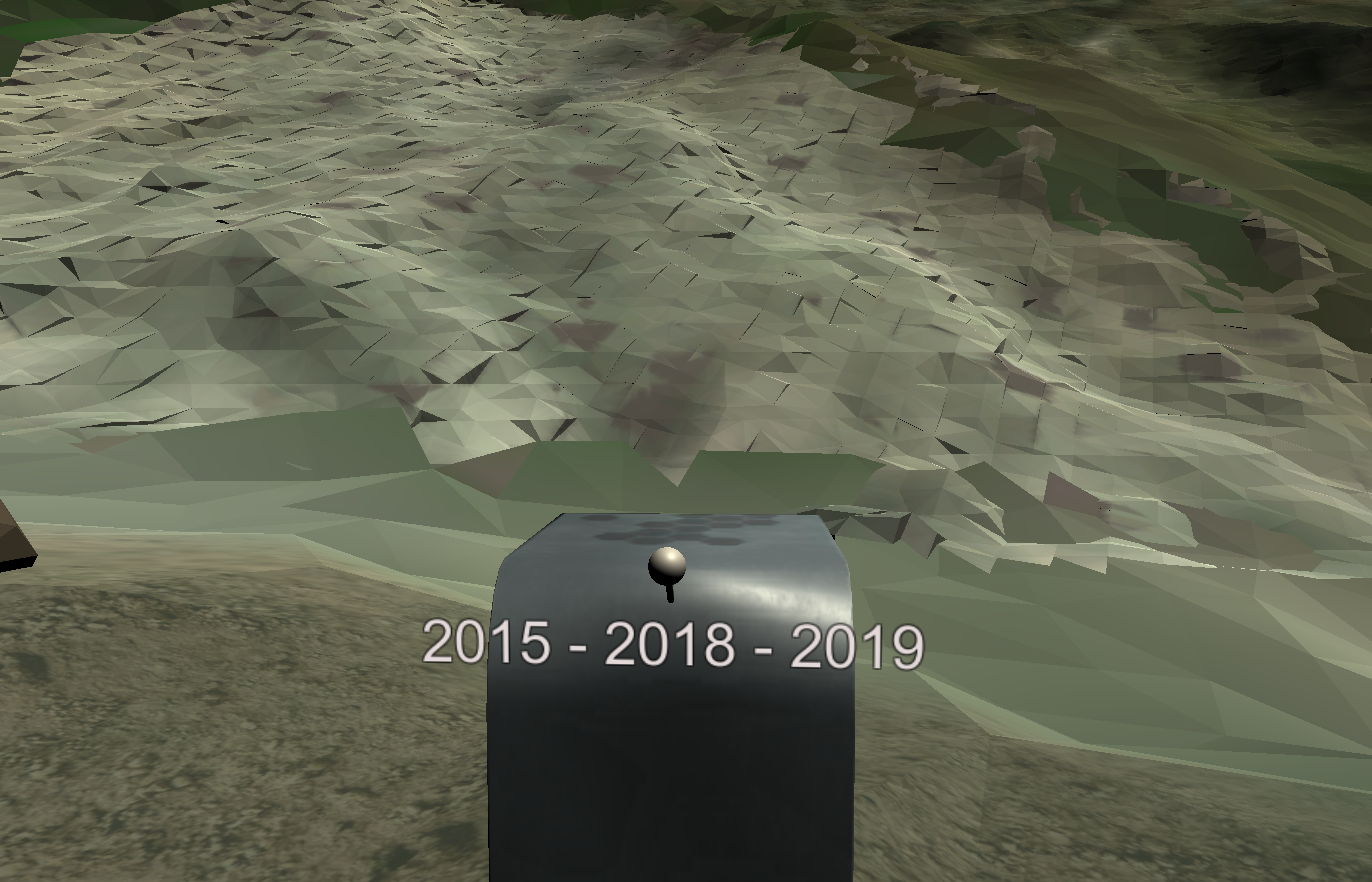
\includegraphics[width=\ImageWidth]{figures/landslide_handler_2.PNG}
            \caption{The Interface for Choosing Landslide Models}
            \label{fig:landslide_handler}
        \end{figure}
        \FloatBarrier
        
        \todo{Screenshot video without scene view}
    
    \subsection{Teleporter}
        In order to decrease the amount of cosmetic decoration that had to be done, and to keep the player's interest, the game area was reduced from the whole valley to a part where examples of everything interesting was. This meant however that the player had to travel down a steep 20m high valley side. This would not be ideal for either of the movement options. This was solved by adding a teleporter that sets the position and rotation of the player to the target teleport station. For simplicity it reuses the button from the image viewers, but use a different colour to signal the same usage, but different effect. The teleporter is shown in \cref{fig:teleporter} below:
        
        \FloatBarrier
        \begin{figure}
            \centering
            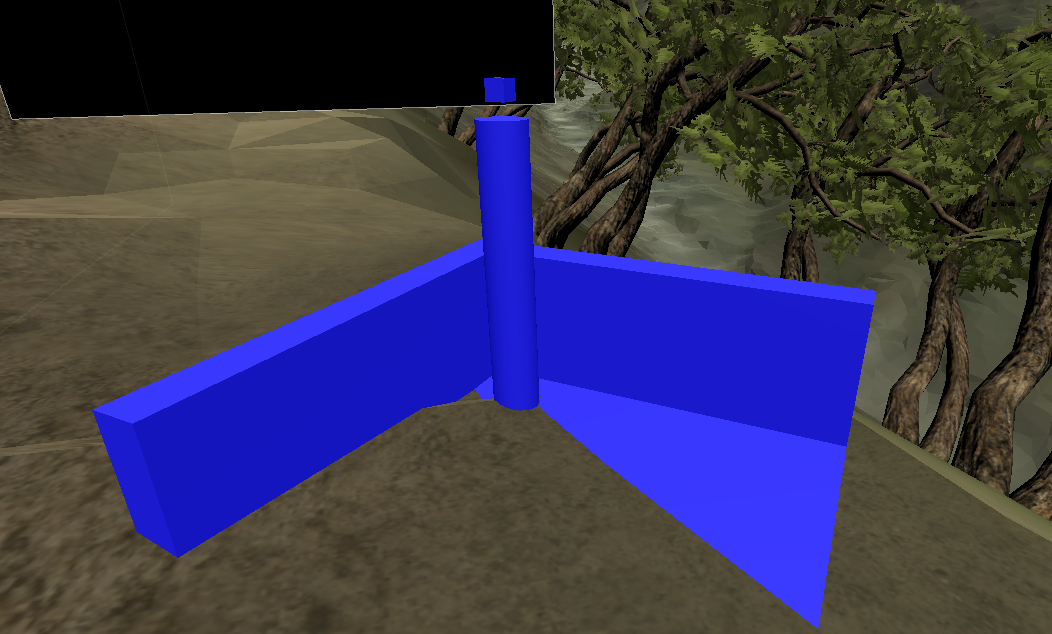
\includegraphics[width=\ImageWidth]{figures/teleporter.PNG}
            \caption{The Teleporter for Moving the PLayer}
            \label{fig:teleporter}
        \end{figure}
        \FloatBarrier
    
    \subsection{Toggling Trees}
        A feature discovered in early prototype testing was the ability to toggle the trees on and off. The trees were added as an aesthetic, but the shape of the valley itself can be of interest in geography. So a button was introduced that sets the parent of the trees, and therefore all the children, to active or inactive. Like the teleporter, it reuses the button from the image viewer, but with a different colour, as shown below in \cref{fig:toggle_tree}.
        
        \FloatBarrier
        \begin{figure}
            \centering
            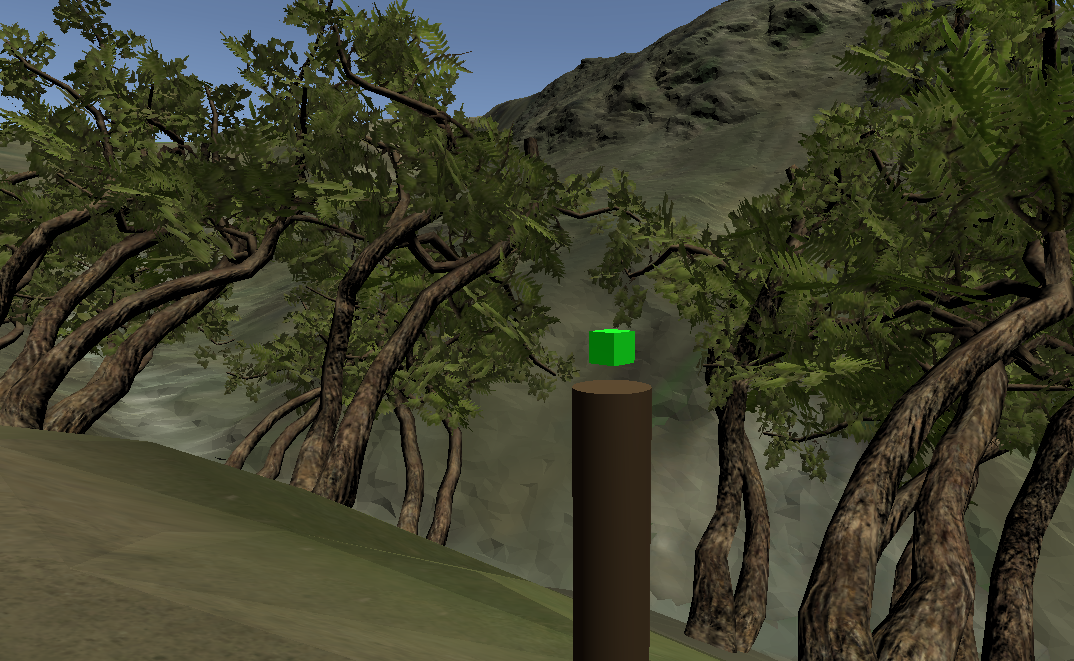
\includegraphics[width=\ImageWidth]{figures/toggel_trees.PNG}
            \caption{Butt for Toggling the Tree Models}
            \label{fig:toggle_tree}
        \end{figure}
        \FloatBarrier
    
    \subsection{Decorating the Game World}
        In order to make the application more engaging and lifelike, models of trees, grass and stones were added to areas where they appear in real life. Additionally, as the satellite photograph used to texture the area only looks good at a distance, the main game area was re-textured. The tool for both of these aesthetic changes was Polybrush\cite{polybrush}. It is tool for Unity available for free that is used to paint with textures and place models on the surface of other models.

\section{Achieved Milestones}
    % A table documenting achieved milestones: when and what
    To document the progress, different milestones with dates are noted in the following table:
    
    \FloatBarrier
    \begin{table}[htbp]
        \centering
        \begin{tabular}{|c|p{0.8\linewidth}|}
            \hline
            \textbf{Date} & \textbf{Milestone} \\
            \hline
            2020-01-15 & Meeting with domain experts to show progress and plans \\
            2020-02-04 & Finished ground models \\
            2020-02-06 & Meeting with domain expert to discuss interaction elements and content to be included \\
            2020-02-13 & Supervisor meeting to discuss research questions and gameplay elements \\
            2020-02-25 & User testing of both apps by geography students \\
            2020-02-27 & Domain expert test of application \\
            2020-04-17 & Soft code freeze -- last feature added to code \\
            2020-05-01 & Code freeze -- last fix added to code \\
            2020-05-05 & Distributed application, video and questionnaire \\
            2020-05-08 & Patched bug in code \\
            2020-05-15 & \todo{Performed last interview with domain experts} \\
            2020-05-18 & \todo{Data collection freeze -- no new answers} \\
            \hline
        \end{tabular}
        \caption{Achieved milestones}
        \label{tab:milestones}
    \end{table}
    \FloatBarrier
